\documentclass[12pt]{exam}
\usepackage[utf8]{inputenc}		% Caracteres latinos
\usepackage[spanish]{babel}		% Idioma español
\usepackage{geometry}			% Organizar el documento
\usepackage{graphicx}			% Incluir gráficos
\usepackage{makecell}			% Para personalizar las celdas de una tabla
\usepackage[nohdr]{mathexam}	% Añadimos el paquete mathexam (sin header)
\usepackage{amsmath}
\usepackage{amsfonts}
\usepackage{amssymb}
\usepackage{mathtools}
\usepackage{tikz,pgfplots}
\usepgfplotslibrary{polar}
\usepackage[shortlabels]{enumitem}
 \renewcommand{\baselinestretch}{1.5}
\usepackage{mathtools}
\usepackage{bm}
\usepackage{esvect}
\usepackage[fleqn]{mathtools}
\usepackage{relsize}
\usepackage{multirow}
\usepackage{multicol}
\usepackage[document]{ragged2e}
 \usepackage{textpos}
\usepackage{tcolorbox}
\usepackage{hyperref}
\usepackage{mathdesign}


% Definimos la geometría de la primera página
\geometry{
	a4paper,                    % Tamaño del documento
	hmargin = {1.7cm, 1.6cm}, 	% Margen horizontal izquierdo, derecho
	vmargin = {1cm, 1cm},	    % Margen vertical superior, inferior
	headsep = 4mm,				% Separación entre el encabezado y el texto
	head = .2cm,				% Tamaño del encabezado
	% marginparsep = 5mm, 		% Seperación entre las notas y el texto
	% marginpar = 1.5cm,		% Tamaño de las notas
	includeall,                 % incluye el encabezado, footer y notas dentro del tamaño del documento
	nomarginpar,	            % Elimina las notas
	foot = 1cm,                 % Tamaño del footer
	twoside,                	% Habilita el modo de impresión a doble cara
}

\selectlanguage{spanish}        % Selecciona el idioma
\spanishdecimal{.}

\newcommand{\iuni}{\pmb{\hat{\imath}}}
\newcommand{\juni}{\pmb{\hat{\jmath}}}
\newcommand{\kuni}{\pmb{\hat{k}}}
\renewcommand{\sin}{\,\text{sen}\,}
\newcommand*\colvec[3][]{
    \begin{pmatrix}\ifx\relax#1\relax\else#1\\\fi#2\\#3\end{pmatrix}
}
% DOCUMENTO
\begin{document}

\centering


\Large 
\textbf{\huge Reposición 1 \\ \large }

\small
\vskip10pt
\normalsize

\pointpoints{punto}{puntos}
\pointformat{\bfseries\boldmath(\thepoints)}
\vskip10pt

    
    \begin{questions}
     \question
     Identifica la ecuación con su campo correspondiente. \textbf{Justifica} tu elección.
     
     \begin{tabular}{llll}
       i) $\frac{dy}{dx}=x-1$   & ii) $\frac{dy}{dx}=1-y^2$ & iii) $\frac{dy}{dx}=y^2-x^2$ & iv) $\frac{dy}{dx}=1-x$ \\
         v) $\frac{dy}{dx}=1-y$ & vi) $\frac{dy}{dx}=x^2-y^2$ & vii) $\frac{dy}{dx}=1+y$ & viii) $\frac{dy}{dx}=y^2-1$
     \end{tabular}
     
     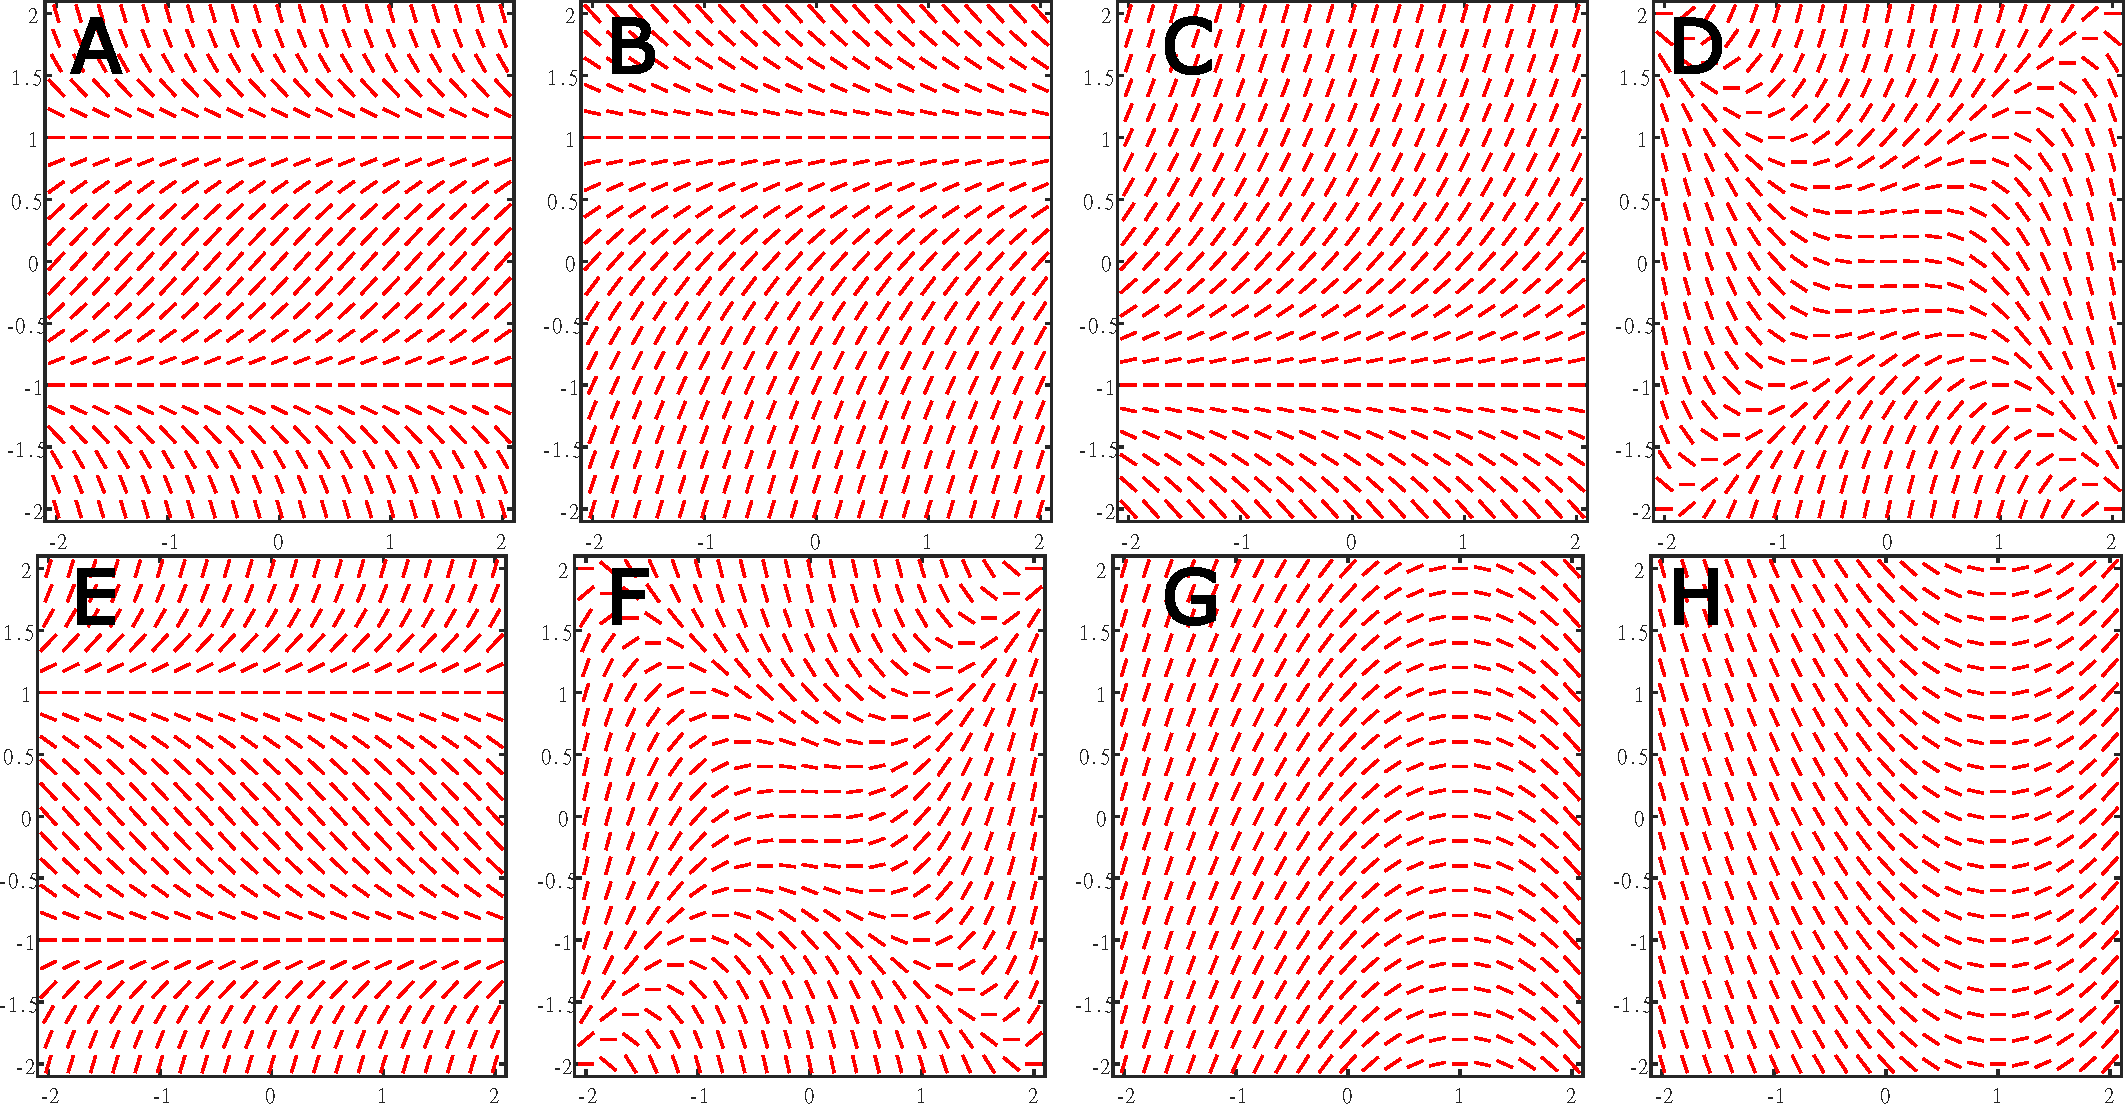
\includegraphics[scale=.48]{F1T1.pdf}
     \question
     El modelo de una cierta población esta descrito por una ecuación diferencial $dP/dt=f(P)$, donde $P(t)$ es la población al tiempo $t$ y de la cual se ha recabado la siguiente información:
     
     \begin{itemize}
         \item Se encontraron puntos de equilibrio solamente en $P=0$, $P=10$ y $P=50$.
         \item Cuando la población es igual a 100, ésta decrece.
         \item Cuando la población es igual a 25, ésta incrementa.
     \end{itemize}
     
     \begin{enumerate}[a)]
         \item Esboza las dos posibles líneas fases del sistema para $P>0$.
         \item Esboza las correspondientes funciones $f(P)$ para cada una de las líneas fase.
         \item Da una fórmula para la función $f(P)$ cuyas gráficas coincidan \textbf{cualitativamente} con las gráficas de \textbf{b)} para cada una de las líneas fase.
     \end{enumerate}

     
     \question
     La ley de Stefan de la radiación establece que la tasa de cambio de temperatura de un cuerpo a $T(t)$ Kelvin en un medio a $M(t)$ Kelvin es proporcional a $M^4-T^4$. Es decir, $$\frac{dT}{dt}=K\left[M^4(t)-T^4(t) \right],$$ donde $K=2.9\times10^{-10}(\text{min})^{-1}$ y $M(t)=293$ Kelvin. Si $T(0)=360$ Kelvin, usa el método de Euler con $h=3\,\text{min}$ para aproximar la temperatura del cuerpo después de:
     
     \begin{enumerate}[a)]
         \item 30 minutos
         \item 60 minutos
     \end{enumerate}


     \question
     Identifica la ecuación como homogénea, de Bernoulli, con coeficientes lineales o de la forma $y'=G(ax+by)$. Resuelve las ecuaciones.
     \begin{enumerate}[a)]
        \item $(2x-y)dx+(4x+y-3)dy=0$
        \item $\frac{dx}{dt}+tx^3+\frac{x}{t}=0$
        \item $\frac{dy}{dx}= \sin(x-y)$
     	\item $(y-4x-1)^2dx-dy=0$
        \item $2tx\,dx+(t^2-x^2)dt=0$
       \end{enumerate}

     \question
     Según la ley de enfriamiento de Newton, al introducir un objeto a temperatura $T$ en un medio con temperatura $M$, la razón de cambio de $T$ es proporcional a la diferencia de temperatura $M-T$ siguiendo la ecuación diferencial $\frac{dT}{dt}=k(M-T)$:
     \begin{enumerate}[a)]
     \item	Resuelve la ecuación diferencial en términos de $T$
     \item	Si un termómetro marca $100°F$ y se coloca en un medio con temperatura constante de $70°F$.  Después de 6 min el termómetro marca $80°F$. ¿Cuál es la lectura después de 20 minutos?
     \end{enumerate}


     \question
     Supón que una solución salina con 0.2 kg de sal por litro se introduce en un tanque que contiene inicialmente 500 litros de agua y 5 kg de sal. La solución entra al tanque a razón de 5 L/min. La mezcla se mantiene uniforme revolviéndola, y sale del tanque a razón de 5 L/min.

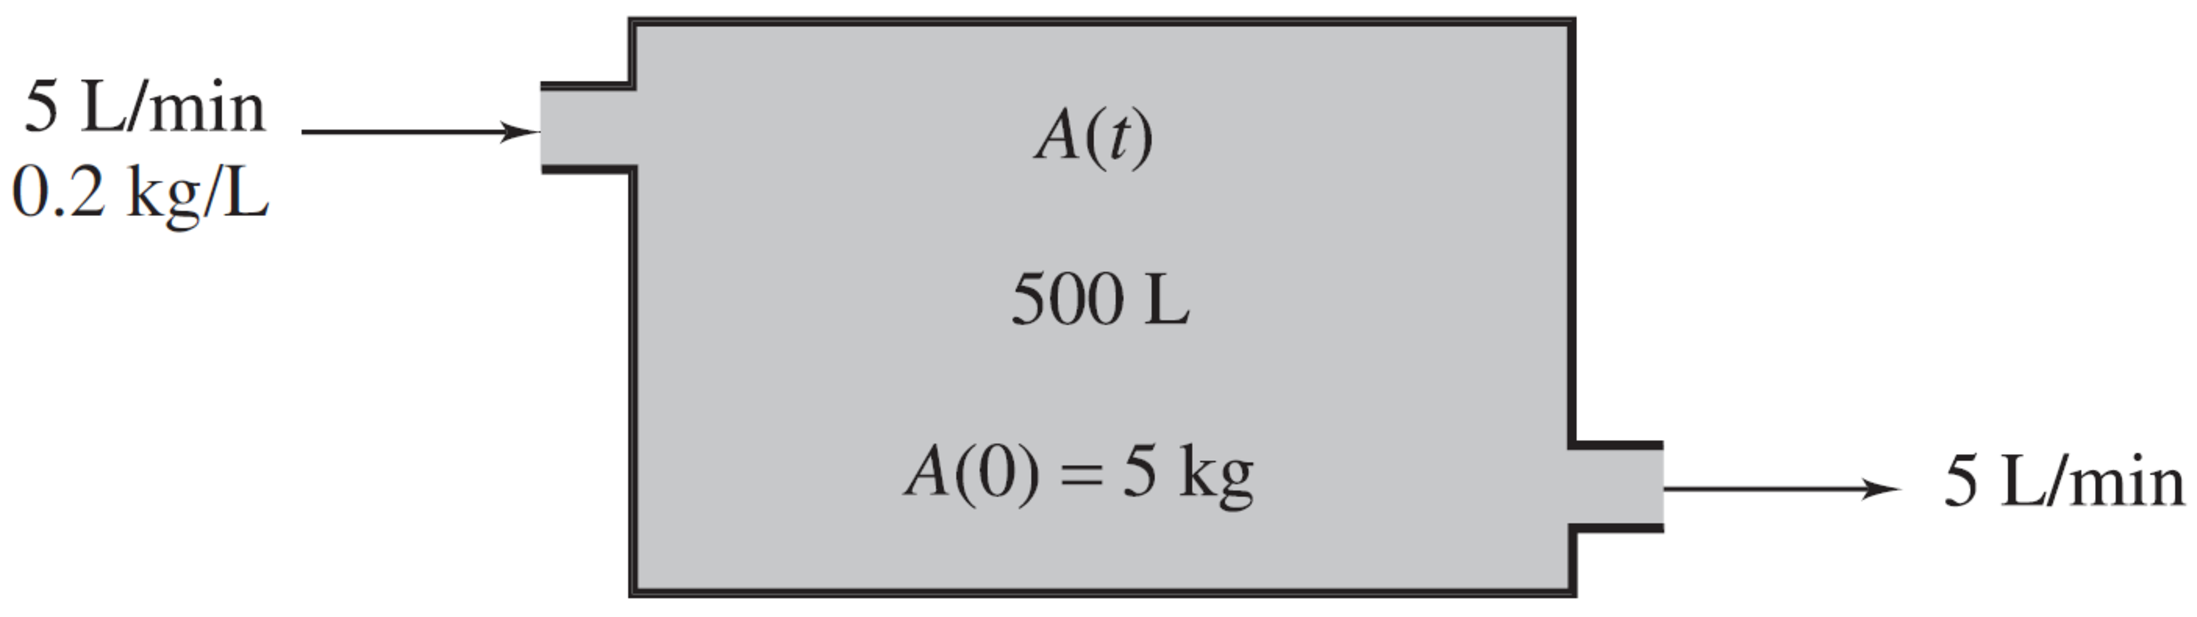
\includegraphics[scale=.34]{F2T2.pdf}

\begin{enumerate}[a)]
	\item	Determina la concentración en kilogramos/litros de sal en el tanque después de 10 minutos viendo al modelo como una ecuación lineal.
    \item Después de 10 minutos aparece en el tanque una fuga a razón de 1 L/min. ¿Cuál será la concentración (en kg/L) de sal en el tanque después de 20 minutos a partir del inicio de la fuga?
    
    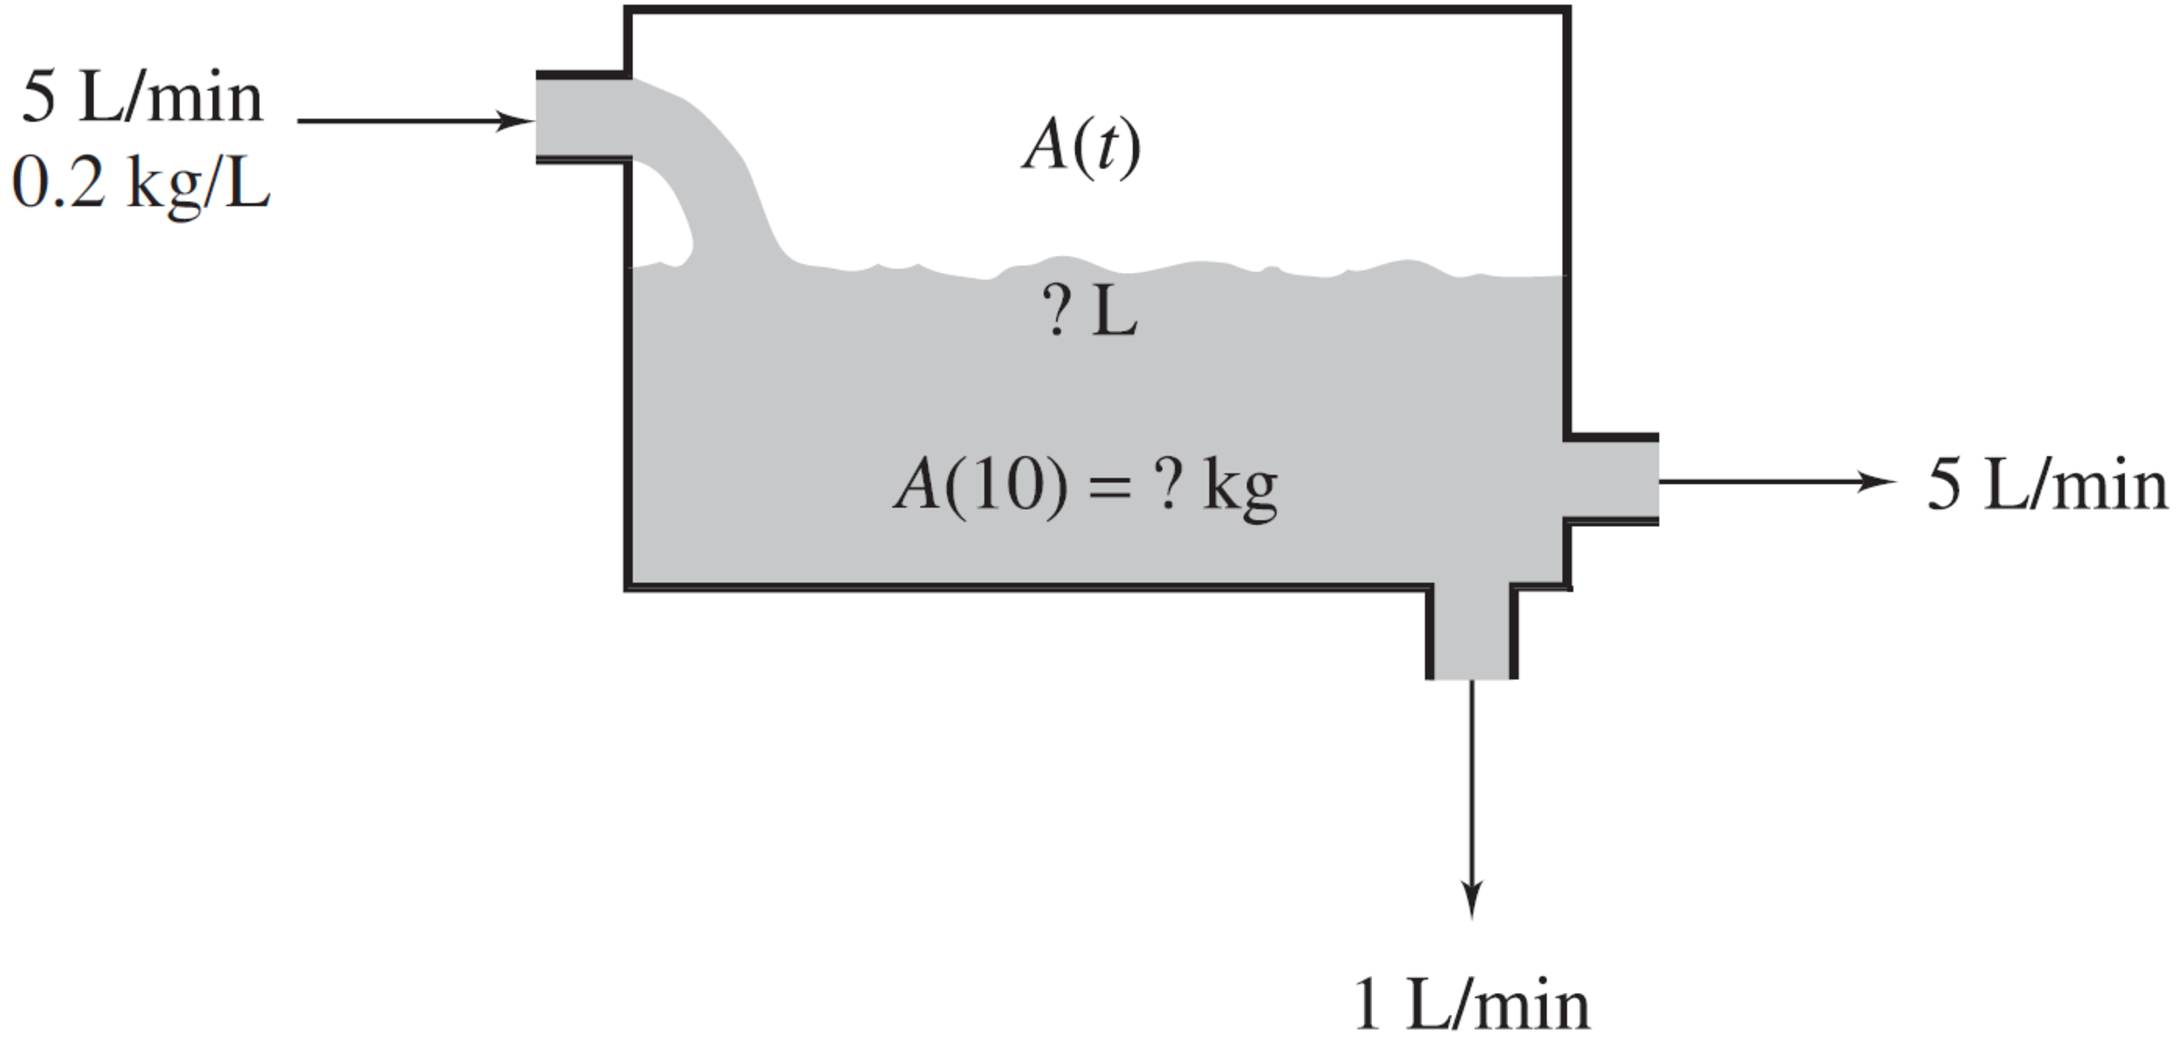
\includegraphics[scale=.34]{F3T2.pdf}
 \end{enumerate}


     \question
      Si las siguiente ecuaciones son exacta, resuélvelas.
      \begin{enumerate}[a)]
      	\item	$e^t(y-t)dt+(1+e^t)dy=0$
        \item	$(\tan y-2)dx+(x\sec^2y+1/y)dy=0$, con $y(0)=1$
      \end{enumerate}

     \question
     Para cada una de las siguientes ecuaciones, determina la función más general $M(x,y)$ de modo que la ecuación sea exacta:
     \begin{enumerate}[a)]
     	\item	$M(x,y)dx+(\sec^2y-x/y)dy=0$
        \item	$M(x,y)dx+(\sin x\cos y-xy-e^{-y})dy=0$
     \end{enumerate}

        \end{questions}

\end{document}
